\documentclass[12pt]{article}

\usepackage[english]{babel}
\usepackage[utf8x]{inputenc}
\usepackage{amsmath}
\usepackage{enumitem}
\usepackage{graphicx}
\usepackage{ulem}
\usepackage{caption}
\usepackage{placeins}
\usepackage[usenames,dvipsnames]{color}
\usepackage[colorinlistoftodos]{todonotes}
\usepackage{listings}
\usepackage{fixltx2e}
\usepackage{scrpage2}
\usepackage{lastpage}
\clearscrheadfoot
\pagestyle{scrheadings}
\usepackage{glossaries}
\usepackage[
top    = 2.75cm,
bottom = 2.00cm,
left   = 2.50cm,
right  = 2.00cm]{geometry}
\setcounter{secnumdepth}{4}
\definecolor{dkgreen}{rgb}{0,0.6,0}
\definecolor{gray}{rgb}{0.5,0.5,0.5}
\definecolor{mauve}{rgb}{0.58,0,0.82}

\newcommand{\executeiffilenewer}[3]{%
\ifnum\pdfstrcmp{\pdffilemoddate{#1}}%
{\pdffilemoddate{#2}}>0%
{\immediate\write18{#3}}\fi%
}
\newcommand{\includesvg}[1]{%
\executeiffilenewer{#1.svg}{#1.pdf}%
{inkscape -z -D --file=#1.pdf --export-pdf=#1.pdf --export-latex}%
\input{#1.pdf_tex}%
}

\lstset{frame=tb,
  language=Java,
  aboveskip=3mm,
  belowskip=3mm,
  showstringspaces=false,
  columns=flexible,
  basicstyle={\small\ttfamily},
  numbers=none,
  numberstyle=\tiny\color{gray},
  keywordstyle=\color{blue},
  commentstyle=\color{dkgreen},
  stringstyle=\color{mauve},
  breaklines=true,
  breakatwhitespace=true
  tabsize=3
}

\makeglossaries

\newglossaryentry{glossaryVerweis} {name=abkuerzung, description={Langer Name}}


\begin{document}
\begin{titlepage}
\begin{center}
% Oberer Teil der Titelseite:

\includegraphics[width=0.5\textwidth]{images/logo}\\[1cm]    

\textsc{\LARGE Technologisches Gewerbe Museum}\\[1.5cm]

% Title
\rule{12cm}{1mm}
{ \huge \bfseries  \\ \huge I2C \\ \large SYT IndInf\\[0.4cm] }

\rule{12cm}{1mm}

% Author and supervisor
\noindent 
\vspace{5cm}

\begin{center}
\large
Siegel Hannah 
\end{center}

\vfill

% Bottom of the page
{\large \today}

\end{center}
\end{titlepage}

\tableofcontents


%HEADER AND FOOTER
\pagenumbering{arabic}
\ohead{\headmark}
\automark{section}
\ifoot{© Authors}
\ofoot{\pagemark ~of \pageref{LastPage}}

\newpage


\section{Task Description}
A project should be done, where the ADXL345 Sensor is sending Informations to the Controller using I2C.
The 3 axes should be printed out using UART. 
\subsection{Team}
We (Wolfang Mair, Christian Janeczeck and Andreas Vogt) met on Saturday, 10.01.2015 as a Team in the School. \\
We did the example together, because we were not able to do it by ourselves and we only had one Sensor (ADXL345).
Therefore we started the example together. We have done it in this team, and the Code is not a copy from anybody else from our class. We have also all understood I2C. The code is not exactly the same, but it may be quite the same. \\
We thought, that it would be fine if we would form a team, and we hope that this is not a problem. We are happy to show the program working on each our stations if required to proove that we have all done it equally.
Every Person from the Team has commented the source code by themselves, done the protocol by their own and finalized to code.
\section{Working time}
\begin{center}
\textbf{Estimated working time}
\end{center}
\begin{table}[h]
\begin{tabular}{|p{0.4\textwidth}|p{0.2\textwidth}|}
\hline
\textbf{Task}                                              & \textbf{Time in hours                              } \\ \hline \hline
Setting up the working environments &  1  \\ \hline 
Running any example &  1  \\ \hline 
UART &  1  \\ \hline 
I2C Implementation &  4  \\ \hline 
Debuging \& Testing &  10  \\ \hline 
Documentation &  1  \\ \hline 
\hline
Total &  17 hours \\ \hline 
\end{tabular}
\end{table}
\begin{center}
\textbf{Final working time}
\end{center}
\begin{table}[h]
\begin{tabular}{|p{0.4\textwidth}|p{0.2\textwidth}|}
\hline
\textbf{Task}                                              & \textbf{Time in hours                              } \\ \hline \hline
Setting up the working environments &  1  \\ \hline 
Running any example &  0.5  \\ \hline 
UART &  3  \\ \hline 
I2C Implementation &  4 \\ \hline 
Debuging \& Testing & 3  \\ \hline 
Documentation &  2  \\ \hline 
\hline
Total &  13 hours \\ \hline 
\end{tabular}
\end{table}


\section{Working protocol}
\subsection{How to connect the ADXL345}
\textbf{Voltage Supply} \\
"I2C and SPI digital communications are available. In both cases,
the ADXL345 operates as a slave. I2C mode is enabled if the CS
pin is tied high to VDD I/O. [..] ",\cite[page 15]{datasheetADXL}
\\ \\
\textbf{Voltage Supply} \\
" With CS tied high to VDD I/O, the ADXL345 is in I2
C mode, requiring a simple 2-wire connection, as shown in Figure \ref{fig:i2clayout} ",\cite[page 18]{datasheetADXL}. I connected the Clock with PB2 and the Data with PB3. I also connected the Voltage Supply with the +3.3V and the Ground to the controllers GND port.
\begin{figure}[here!]
\centering
    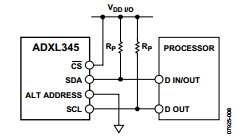
\includegraphics[width=0.4\textwidth]{images/i2clayout}
    \caption{I2C Layout \cite[page 18]{datasheetADXL}}
    \label{fig:i2clayout}
\end{figure}
\begin{figure}[here!]
\centering
    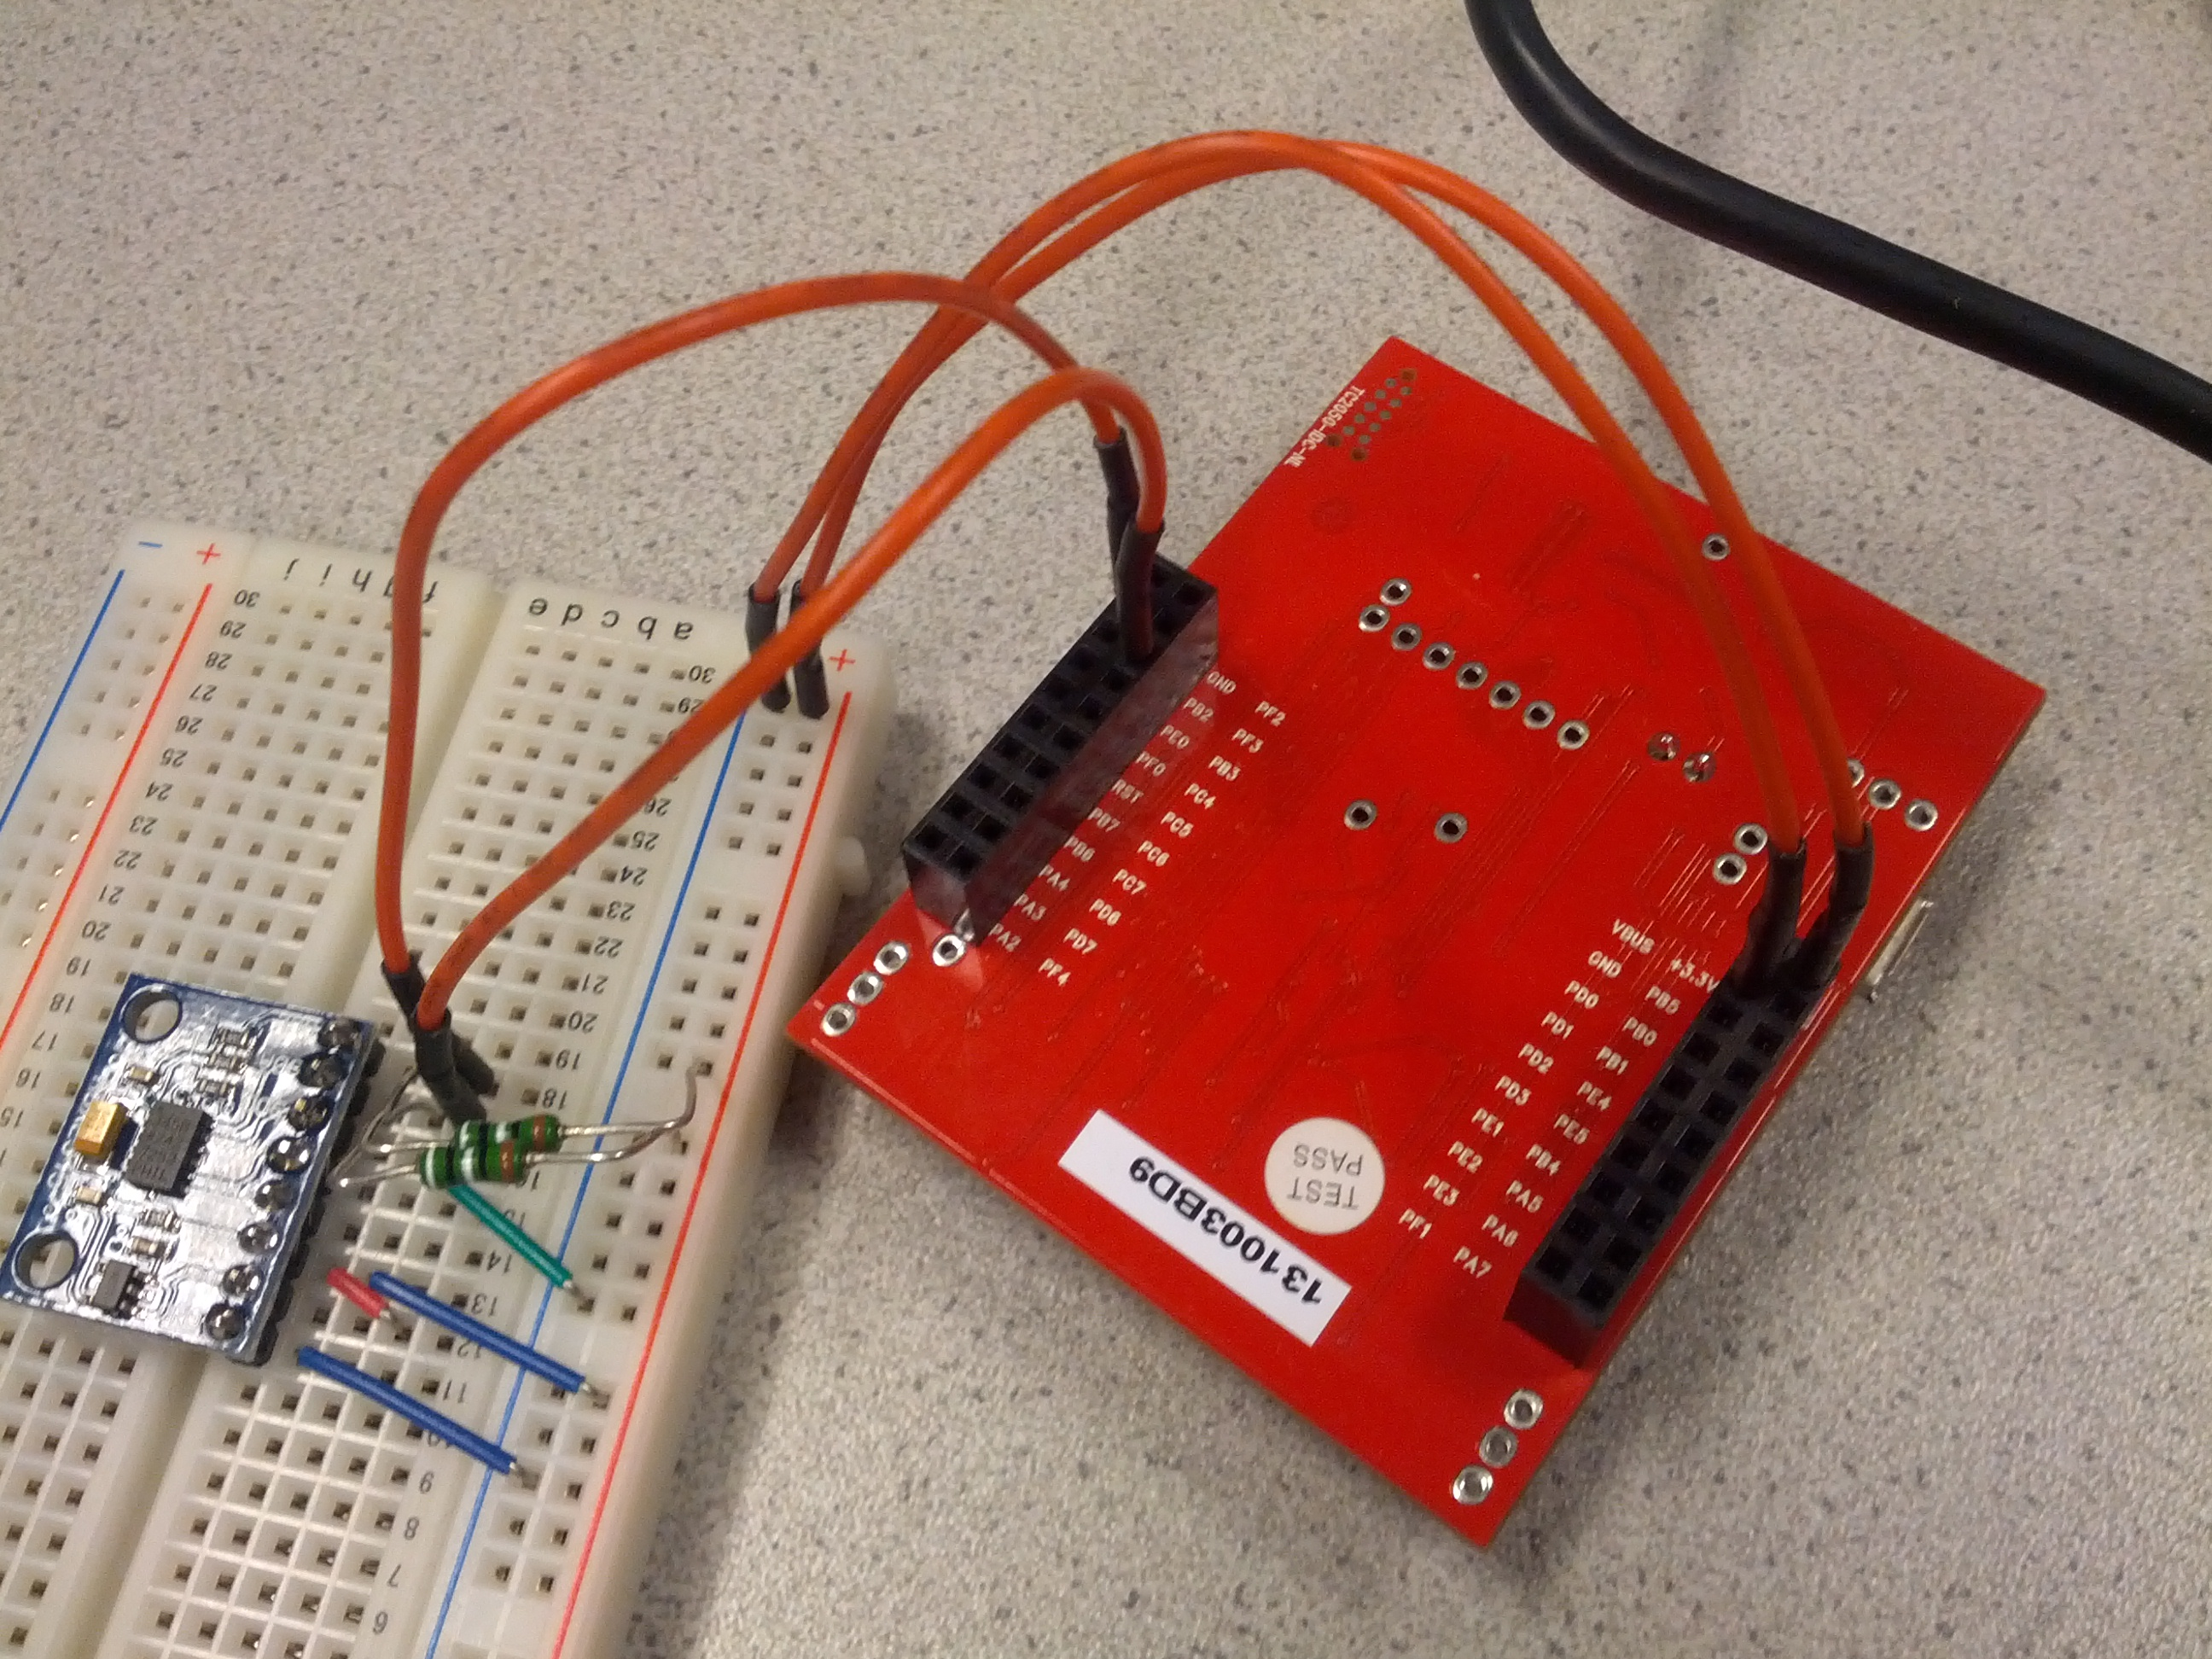
\includegraphics[width=0.4\textwidth]{images/con2}
    \caption{How to connect the wires}
    \label{fig:i2clayout2}
\end{figure}
\subsection{Setting up the working environement}
I used the DebianVM we got in VMWare-Workstation. The Makefile could be found in the tiva-template \cite{tivatemp}. At first I copied it into the github-repo. I also copied the \texttt{TM4C123GH6PM.ld} File.
\\ I than copied the Files from the \texttt{/home/schueler/opt/tivaware/examples/peripherals/i2c} into the repository and changed the Makefile. I set the PROJ simply to src: \texttt{PROJ := src}. 
\newpage
\subsection{UART}
I than added only the UART.  I wrote a method called \texttt{UARTConf}. In it, the necessary configurations for UART were done. 
\begin{lstlisting}    
extern void UARTConf(void) {
   // Enable Ports for UART
   ROM_SysCtlPeripheralEnable(SYSCTL_PERIPH_GPIOA);
   ROM_SysCtlPeripheralEnable(SYSCTL_PERIPH_UART0);

   // Enable A0 and A1 for UART pins
   ROM_GPIOPinConfigure(GPIO_PA0_U0RX);
   ROM_GPIOPinConfigure(GPIO_PA1_U0TX);
   ROM_GPIOPinTypeUART(GPIO_PORTA_BASE, GPIO_PIN_0 | GPIO_PIN_1);

   // Set Clock Source
   UARTClockSourceSet(UART0_BASE, UART_CLOCK_PIOSC);

   // Config UART
   UARTStdioConfig(0, 115200, 16000000);
}
\end{lstlisting}    
I than commented all the I2C parts out, only to test UART. 
I used \texttt{cutecom} to read the UART output. Somehow the UART didn't work.  \\
I tried for a long time and finally we found an example in tivaware-template \cite{tivatemp},  \texttt{buttons\_isr}.
I changed the Makefile in the tiva-template so that this class will be executed. And here the UART worked fine.
So I decided to simply use the \texttt{buttons\_isr} as a scaffold. So everything that has something to do with the buttons was removed. The UART worked fine.
\\ \\
Later, while testing the I2C already, it stopped suddenly working, without that I had changed something. A restart of the system, the \texttt{cutecom} and plugging in and out the micro controller finally did work.  

\newpage
\subsection{I2C}
\subsubsection{Addresses}
"An alternate I2C address of 0x53", \cite[page 18]{datasheetADXL}. This means that the slave address can be found on 0x53. All the other addresses can be found on \cite[page 22]{datasheetADXL}:
\begin{lstlisting}    
0x00 0 DEVID R 11100101 Device ID
0x2D 45 POWER_CTL R/W 00000000 Power-saving features control
0x31 49 DATA_FORMAT R/W 00000000 Data format control
0x32 50 DATAX0 R 00000000 X-Axis Data 0
0x33 51 DATAX1 R 00000000 X-Axis Data 1
0x34 52 DATAY0 R 00000000 Y-Axis Data 0
0x35 53 DATAY1 R 00000000 Y-Axis Data 1
0x36 54 DATAZ0 R 00000000 Z-Axis Data 0
0x37 55 DATAZ1 R 00000000 Z-Axis Data 1
\end{lstlisting}    
\subsubsection{Basic I2C Communication}
On page 315 and following it is explained how the I2C must be implemented. \cite[page 315-334]{UG}
\\
\begin{enumerate}
\item The code for setting up the InitI2C was taken from the \texttt{master\_slave\_loopback.c} example.
I did not copy the \texttt{HWREG} line, because it was not working. Also all the loopback settings were not copied. \\
Vennesa then told me, that I had to add the command \texttt{GPIOPinTypeI2CSCL} as well, so I did.
\begin{lstlisting}    
extern void I2CConf(void){
   // Enable the Ports
   SysCtlPeripheralEnable(SYSCTL_PERIPH_I2C0);
   SysCtlPeripheralEnable(SYSCTL_PERIPH_GPIOB);

   // Configure Port B2 onto the Clock
   GPIOPinConfigure(GPIO_PB2_I2C0SCL);

   // Configure Port B3 onto the Data
   GPIOPinConfigure(GPIO_PB3_I2C0SDA);

   // Configure Port B 
   GPIOPinTypeI2C(GPIO_PORTB_BASE, GPIO_PIN_2 | GPIO_PIN_3);

   // Configure Port B for the Clock
   GPIOPinTypeI2CSCL(GPIO_PORTB_BASE, GPIO_PIN_2);

   // Set up the I2C Clock
   I2CMasterInitExpClk(I2C0_BASE, SysCtlClockGet(), NORMAL_CLK);
}
\end{lstlisting} 
\item "the user must first initialize the I2C master
module with a call to \texttt{I2CMasterInitExpClk()}",\cite[page 315]{UG} 
\begin{lstlisting}  
   I2CMasterInitExpClk(I2C0_BASE, SysCtlClockGet(), false);
   \end{lstlisting}    
\cite[page 343]{UG}

\item "Data is transferred by first setting the slave address using \texttt{I2CMasterSlaveAddrSet()}.
",\cite[page 315]{UG} I set the Slave Adress to 0x53, because this was what I have found out previously. "That function
is also used to define whether the transfer is a send (\texttt{write = false, read = true})",\cite[page 315]{UG}
\begin{lstlisting}  
I2CMasterSlaveAddrSet(I2C0_BASE, 0x53, false);
   \end{lstlisting}    
   
   \item "Then, if connected to an I2C bus that has multiple
masters, the Tiva I2C master must first call \texttt{I2CMasterBusBusy()} before attempting to initiate the
desired transaction.",\cite[page 315]{UG} But because I only have one master this is not needed. 
\begin{lstlisting}  
    while(I2CMasterBusy(I2C0_BASE)) {}
     \end{lstlisting}    
     
        \item "After determining that the bus is not busy, if trying to send data, the user must
call the \texttt{I2CMasterDataPut()} function. ",\cite[page 315]{UG} First I wanted to read the slave ID.
\begin{lstlisting}  
I2CMasterDataPut(I2C0_BASE, 0x00);
\end{lstlisting}  
     
\item "After determining that the bus is not busy, if trying to send data, the user must
call the \texttt{I2CMasterDataPut()} function. ",\cite[page 315]{UG} First I wanted to read the slave ID.
\begin{lstlisting}  
I2CMasterDataPut(I2C0_BASE, 0x00);
\end{lstlisting}  
      

\item "The transaction can then be initiated on the bus by calling
the \texttt{I2CMasterControl()} function with any of the following commands: \\
\texttt{I2C\_MASTER\_CMD\_SINGLE\_SEND} \\
\texttt{I2C\_MASTER\_CMD\_SINGLE\_RECEIVE} \\
\texttt{I2C\_MASTER\_CMD\_BURST\_SEND\_START} \\
\texttt{I2C\_MASTER\_CMD\_BURST\_RECEIVE\_START}."
,\cite[page 315]{UG} \\ I used the \texttt{I2C\_MASTER\_CMD\_SINGLE\_SEND} command.
\begin{lstlisting}  
    I2CMasterControl(I2C0_BASE, I2C_MASTER_CMD_SINGLE_SEND);
\end{lstlisting}  
       
\item "For the single send and receive cases, the polling method involves looping on the return from
\texttt{I2CMasterBusy()}. ",\cite[page 316]{UG} 
\begin{lstlisting}  
    while(I2CMasterBusy(I2C0_BASE)) {}
\end{lstlisting} 

  \item " Once that function indicates that the I2C master is no longer busy, the bus trans-
action has been completed and can be checked for errors using \texttt{I2CMasterErr()}. ",\cite[page 316]{UG} 
\begin{lstlisting}  
    int8_t error = I2CMasterErr(I2C0_BASE);
\end{lstlisting} 
                        
     \item " If there are no errors, then the data has been sent or is ready to be read using \texttt{I2CMasterDataGet()}. ",\cite[page 316]{UG} 
\begin{lstlisting}  
    data = (int8_t) I2CMasterDataGet(I2C0_BASE);
\end{lstlisting}    
     
\end{enumerate}
\newpage
  So the complete code is to read a value is:
\begin{lstlisting}    
extern int8_t read(uint32_t slaveAddress, uint32_t registerAddress){
    // Set the Slave Address and write
    I2CMasterSlaveAddrSet(I2C0_BASE, slaveAddress, WRITE);

    // Set the Register / Data to get
    I2CMasterDataPut(I2C0_BASE, registerAddress);

    // Sending
    I2CMasterControl(I2C0_BASE, I2C_MASTER_CMD_SINGLE_SEND); 

    // Waiting until the Master is done
    while(I2CMasterBusy(I2C0_BASE)) {} 

    // Get error code, if there is one
    int8_t error = I2CMasterErr(I2C0_BASE);
    if (error != I2C_MASTER_ERR_NONE){
	UARTprintf("\n error-code : %i \n",error);
    }

    // Set the Slave Address and read
    I2CMasterSlaveAddrSet(I2C0_BASE, slaveAddress, READ);

    // Reiciving Data
    I2CMasterControl(I2C0_BASE, I2C_MASTER_CMD_SINGLE_RECEIVE);

    // Waiting until the Master is done
    while(I2CMasterBusy(I2C0_BASE)) {}

    // Get error code, if there is one
    error = I2CMasterErr(I2C0_BASE);
    if (error != I2C_MASTER_ERR_NONE){
	UARTprintf("\n error-code : %i \n",error);
    }

    // Fetching the Data out of the register
    int8_t data = (int8_t) I2CMasterDataGet(I2C0_BASE);

    // Return the data
    return data;
}
\end{lstlisting}    
With this code, only the Slave's ID was read. (Using 0x00).
\\ \\
For reading the values, the read method could be used, only with different Addresses.
\newpage
\subsubsection{Power Mode}
I wrote a function for the Power Mode.
It first writes a Register (The Register for the Power mode) and then it writes a second value which turned the Power Mode on. \\
\\
'' After VS is applied, the device enters standby mode, where power
consumption is minimized and the device waits for VDD I/O to be
applied and for the command to enter measurement mode to be
received.  (This command can be initiated by setting the measure
bit (Bit D3) in the POWER\_CTL register (Address 0x2D).)"\cite[page 13]{datasheetADXL}. \\
Therefore I set the 0x2D to 0x3F.
\\ Information about the Register 0x2D—POWER\_CTL can also be seen on page 25.
\begin{lstlisting} 
extern void writePowermode(uint32_t slaveAddress,uint32_t registerAddress,uint32_t data){
    // Set the Slave Address and write
    I2CMasterSlaveAddrSet(I2C0_BASE, slaveAddress, WRITE);

    // Send the Register
    I2CMasterDataPut(I2C0_BASE, registerAddress);
   
    // Sending
    I2CMasterControl(I2C0_BASE, I2C_MASTER_CMD_BURST_SEND_START);
 
    // Waiting until the Master is done
    while(I2CMasterBusy(I2C0_BASE)) {}

    // Get error code, if there is one
    int8_t error = I2CMasterErr(I2C0_BASE);
    if (error != I2C_MASTER_ERR_NONE)
		UARTprintf("\n error-code : %i \n",error);

    // Set the Slave Address and write
    I2CMasterSlaveAddrSet(I2C0_BASE, slaveAddress, WRITE);

    // Send the Power Mode Command
    I2CMasterDataPut(I2C0_BASE, data);

    // Sending
    I2CMasterControl(I2C0_BASE, I2C_MASTER_CMD_BURST_SEND_FINISHED);

    // Waiting until the Master is done
    while(I2CMasterBusy(I2C0_BASE)) {}
   
    // Get error code
    error = I2CMasterErr(I2C0_BASE);
    if (error != I2C_MASTER_ERR_NONE)
		UARTprintf("\n error-code : %i \n",error);
}
\end{lstlisting} 

\subsubsection{Reading the Values}
Reading the Values were easy. I used the read method. After having set the power mode, this has not been any problem. I looped in the main method:
\begin{lstlisting} 
while(1){
      // Print the x Values
      UARTprintf("Slave said: X %i \n", shift(read(SLAVE_ADDRESS, DATAX0),read(SLAVE_ADDRESS, DATAX1)));

      // Print the y Values
      UARTprintf("Slave said: Y %i \n", shift(read(SLAVE_ADDRESS, DATAY0),read(SLAVE_ADDRESS, DATAY1)));

      // Print the z Values
      UARTprintf("Slave said: Z %i \n \n ", shift(read(SLAVE_ADDRESS, DATAZ0),read(SLAVE_ADDRESS, DATAZ1)));

      // Sleep
      ROM_SysCtlDelay(ROM_SysCtlClockGet() / 2);
   }
\end{lstlisting} 
The values ware Bitshifted using the shift method:
Markus Klein helped me with this.
\begin{lstlisting} 
extern int16_t shift(int8_t axis1,int8_t axis2){
  return((int16_t) axis2 << 8) | ((int16_t) axis1);
}
\end{lstlisting} 
\newpage
\subsection{Testing}
\begin{figure}[here!]
\centering
    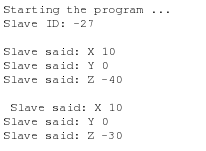
\includegraphics[width=0.4\textwidth]{images/sc1}
    \caption{Startup}
    \label{fig:i2clayout}
\end{figure}

\begin{figure}[here!]
\centering
    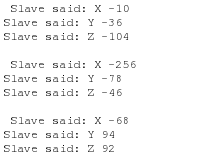
\includegraphics[width=0.4\textwidth]{images/sc2}
    \caption{Some Values}
    \label{fig:i2clayout}
\end{figure}

\begin{figure}[here!]
\centering
    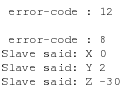
\includegraphics[width=0.3\textwidth]{images/sc3}
    \caption{Errors (I plugged out some wires)}
    \label{fig:i2clayout}
\end{figure}
\FloatBarrier
\newpage
\section{Problems}
\subsection{Build Failed}
Sometimes I received this error message: I was not able to solve it, but it was during using the Loopback example.
\begin{lstlisting}    
build/slave_receive_int.o:/home/schueler/repositories/tiva-template/src/i2c2/slave_receive_int.c:193: first defined here
arm-none-eabi-ld: warning: cannot find entry symbol ResetISR; defaulting to 00000000
Makefile:67: recipe for target 'build/main' failed
make: *** [build/main] Error 1
\end{lstlisting}  
\subsection{Flashing didn't work}
Sometimes I got the following error, even trough the cutecom was able to use the device and the lsusb was showing it. It was solved when plugging out the phone which was charging in the meantime...
\begin{lstlisting}    
lm4flash build/main.bin
Unable to get device serial number: LIBUSB_ERROR_TIMEOUT
Unable to find any ICDI devices
\end{lstlisting}  
\subsection{While loop is not stopping}
I have had the problem that the while-loop within the read() function was an infinite loop, which means that the  Master is always busy. The problem was, that the Voltage cable was not in the port anymore, it was getting out unintended.
\subsection{Are the values correct?}
I had no way to verify the values, and they seemed a little bit odd too, because they were not 0 even trough the sensor was not moving. This problem has not been solved. \\
Also, many students from the class were multiplication the output by 4. \\
I have found the following section in the Datasheet concerning this issue, but to be honest I didnt understand what this precisely means, so I just let the values as they were. \\ \\
"Self-test change is defined as the output (g) when the \texttt{SELF\_TEST} bit = 1 (in the \texttt{DATA\_FORMAT} register, Address 0x31) minus the output (g) when the \texttt{SELF\_TEST} bit = 0. Due to device filtering, the output reaches its final value after 4 × t when enabling or disabling self-test, where t = 1/(data rate). The part must be in normal power operation (\texttt{LOW\_POWER} bit = 0 in the \texttt{BW\_RATE} register, Address 0x2C) for self-test to operate correctly. 
"\cite[page 5]{datasheetADXL}
\subsection{Controller stopped working the next day}
When I tried out the example again the next day, there were no values any more. 
Vennesa told me, that this was because the power mode was not set any more, which means, that the power mode function was not writing as it should have in the first place (because it got set by another code).
The power mode is therefore set for a longer time, which means that the code actually didnt set it and therefore he code was wrong. \\
I solved this bug when I wrote with a \texttt{BURST SEND} instead of the \texttt{SINGLE SEND}.

\begin{thebibliography}{56}
\bibitem{tivatemp} 
  \textbf{Tiva Template Github}, Michael Borko \\
  \textit{https://github.com/mborko/tiva-template}
  \newline last used: 11.01.2015, 10:34  
  
 \bibitem{datasheetADXL} 
  \textbf{Data Sheet ADXL345} \\
  \textit{http://www.analog.com/static/imported-files/data\_sheets/ADXL345.pdf}
  \newline last used: 10.01.2015, 10:36
  
   \bibitem{UG} 
  \textbf{TivaWare™ Peripheral Driver Library} \\
  \textit{https://github.com/mborko/tiva-template/blob/master/docs/SW-TM4C-DRL-UG-2.0.1.11577.pdf}
  \newline last used: 11.01.2015, 10:33
  
 
  
  
\end{thebibliography}
\end{document}
